\chapter{Implemented software}

In order to test the feasibility and to test the speed of the different algorithms different software pieces were needed.

\begin{figure}[H]
\caption{Implemented acquisition software in the CERN infrastructure}
\centering
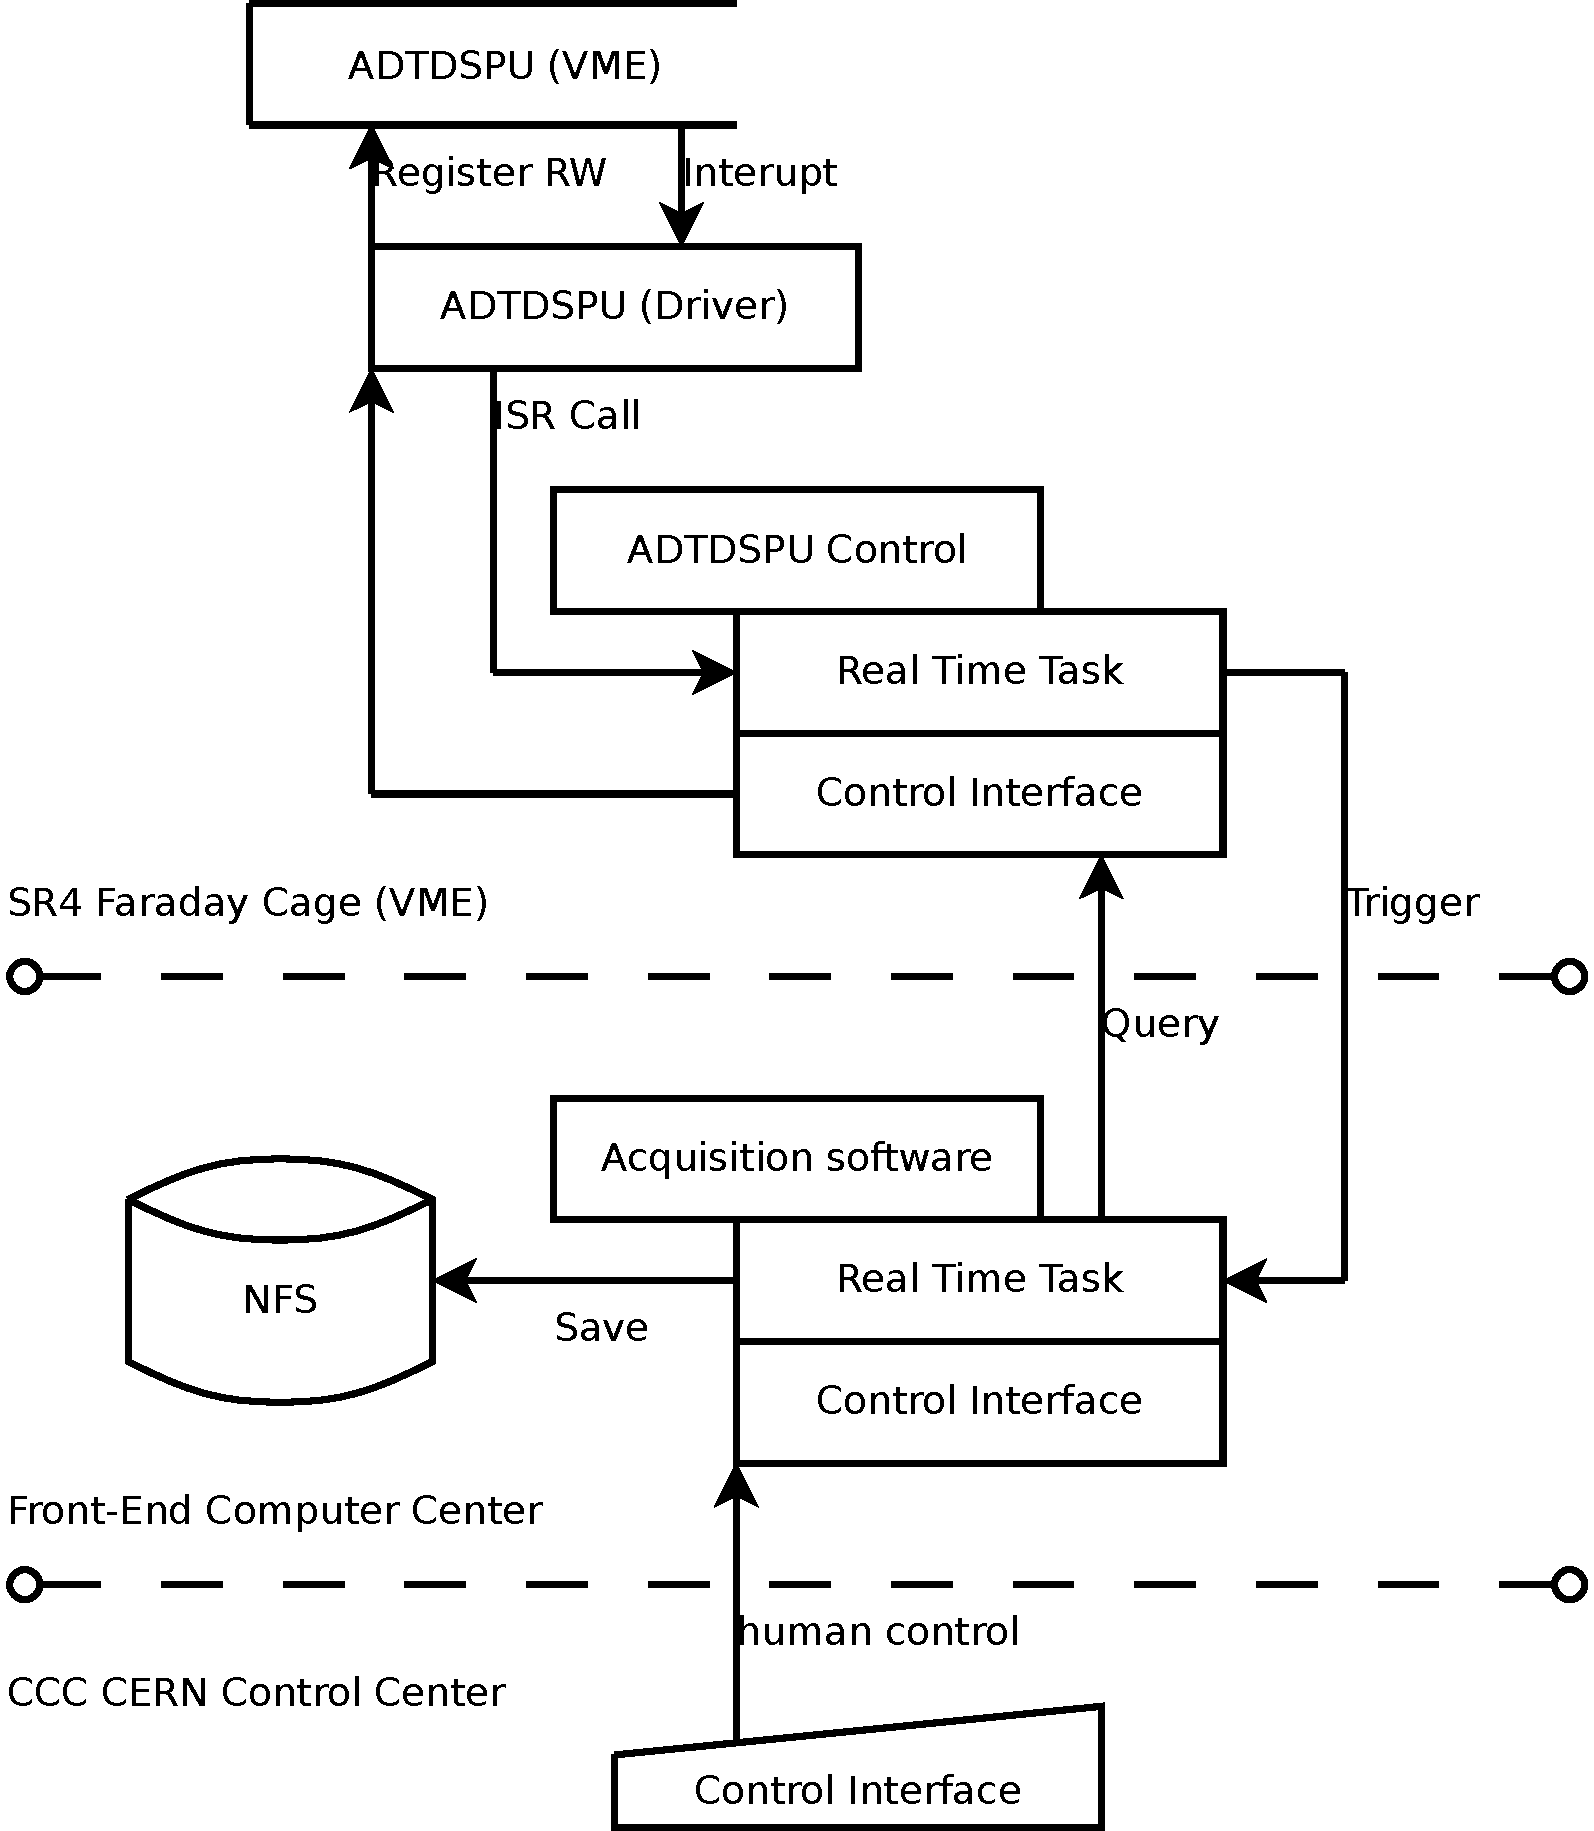
\includegraphics[scale=0.3]{ImplementedSoftFesa.pdf}
\end{figure}

The implemented system consist of three pieces of software~:
\begin{enumerate}
\item The software controlling the acquisition card in the machine.
\item An acquisition software that runs on a standard front-end Linux machine that is taking data during the \glspl{MD}.
\item An analyzing software that can compute the \glspl{FFT} on \glspl{GPU}.
\end{enumerate}

In the final version the software will be merged in a single executable that should run on the machine with the \gls{GPU} and the receiver card. The present solution has been put into place because the present hardware is still in development and there is no way of acquiring the maximum of 2880 bunches from the machine. The hardware is receiving the acquisition data but the \gls{VME} is not fast enough to transfer it to the \gls{CPU}.

\section{ADTDSPU control software}

The first layer that was needed is a driver that can control the \gls{VME} card and forward the interrupts. This is done using the standard driver framework from the \gls{CO} at \gls{CERN}.

The standard \gls{FESA}, the standard middle-ware framework used at \gls{CERN} to control equipments, was used to develop a higher level software to control the card. This particular card needs a real time task in order to react to an interrupt coming from the hardware and to inform when a new acquisition is ready to be read.

The software was originally written by David Gl{\'e}nat, Andrey
Pashnin took it over and wrote the specific part of the ``tune
acquisition'' and is now under Fr{\'e}d{\'e}ric Dubouchet
responsibility together with all other \gls{ADT} software.

It is made of tree main part, two of them user interfaces. The tune
measurement control interface sets the acquisition parameters. The
Tune measurement data receives the data from the card and displays it
to the user. Finally, a real-time task receives the interrupts and
notifies the user that there is new data available.

The Interfaces are exposed trough the \gls{CERN} middle-ware, which
makes it available to other application, such as the data acquisition
software.

\subsection{Control interfaces}

This interface is basic. It allows the user to set the register to
enable the acquisition and to set the mask that decide which bunches
in the acquisition have to be recorded in the memory. The mask is
described as an array of 3564 short (2-bytes word) that can be either
0 (not selected) or 1 (selected).

This interface allow us to select witch bunch we want to acquire. The
machine can never be fully saturated by bunches. A gap is required in
the train to accomodate the extraction kicker risetime, and allow for
the safe dumping of the beam.

Even if the present interface allow us to have the full bunches of the
machine selected, it is clear that as the memory is limited to 16
kilo-short (32 kilo-bytes), we would generate too many interrupts per
second for the interface to be usable.

This interface has two other problems. No double buffering is
implemented, so while the \gls{CPU} is reading values new incoming
values would be lost. Further, the \gls{VME} is too slow to support
the required datarate.

The data interface is the interface the data acquisition software is
using. It provides access to the values from the memory in the
\gls{CPU} as soon as they become available. A system call subscription
used, such that the interface notifies the client software that new
data has become available. It also provides a read back from the
hardware of the various parameters set from the tune measurement
control interface~: the mask and all the controls.

\subsection{Observation memory acquisition}
\label{sec:obs_mem_acq}

\begin{figure}[H]
\caption{ADTDSPU tune acquisition process description}
\centering
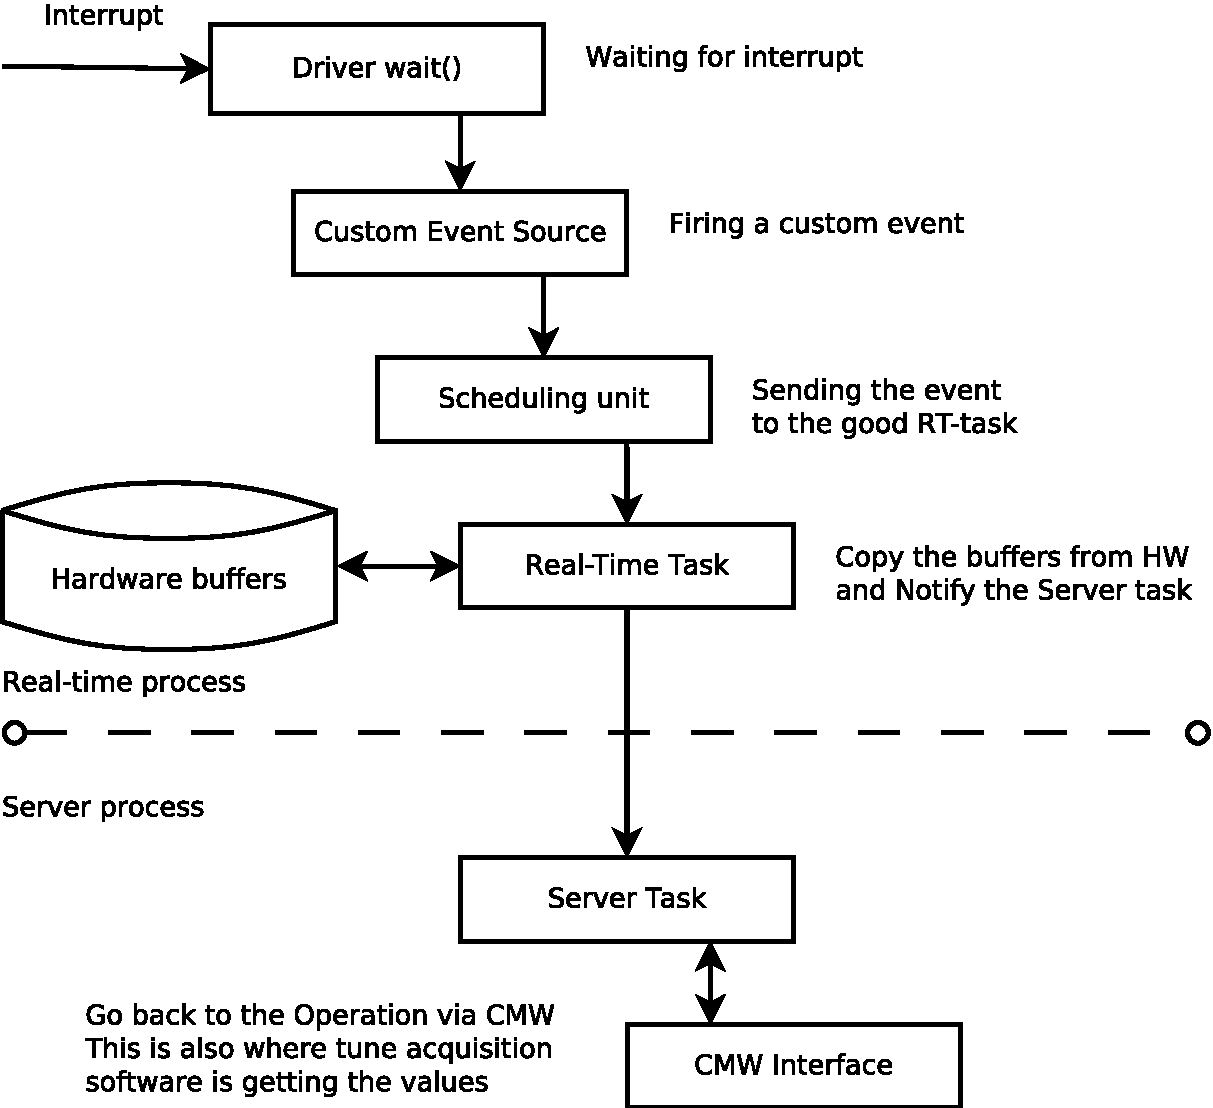
\includegraphics[scale=0.3]{adtdspu_acq.pdf}
\end{figure}

A ``real-time'' process is waiting for the interrupt to happen, using a select like mechanism. The Linux used at \gls{CERN} on the front-ends is a custom kernel with the real-time patch, this guarantees that the latency between the interrupt and the process being called is not too big (usually under 10 micro-seconds).

This process create a custom event sources that trigger the copy of the hardware buffer into the \gls{CPU} buffer and notify the tune measurement data task that the buffers are ready to be read.

Notifying the task actually call it and this task (called server task as this is an interface task) is then telling its clients to come and get the acquisition data. 

\section{Acquisition software}

The acquisition software was used to check that the idea of getting the tune out of the DSPU card data was feasible as well as providing a means to log the acquisition to a file for subsequent checking and processing.

The acquisition software is then able to compute the \gls{FFT} using
\gls{FFTW} and display it to the operators in the \gls{CCC} from where
all the eight accelerators of \gls{CERN} are controlled. On the
interface one can decide which type of graph to display and also
enable saving of the data files to be processed by the data analysis
software.

\subsection{Control interface}

The control interface allow us to decide which file type to save (if we want to save the data to a file), where to save theses data and which ADTDSPU we are subscribing to.

\begin{figure}[H]
\caption{ADTDSPU tune acquisition software interface in the FESA framework}
\centering
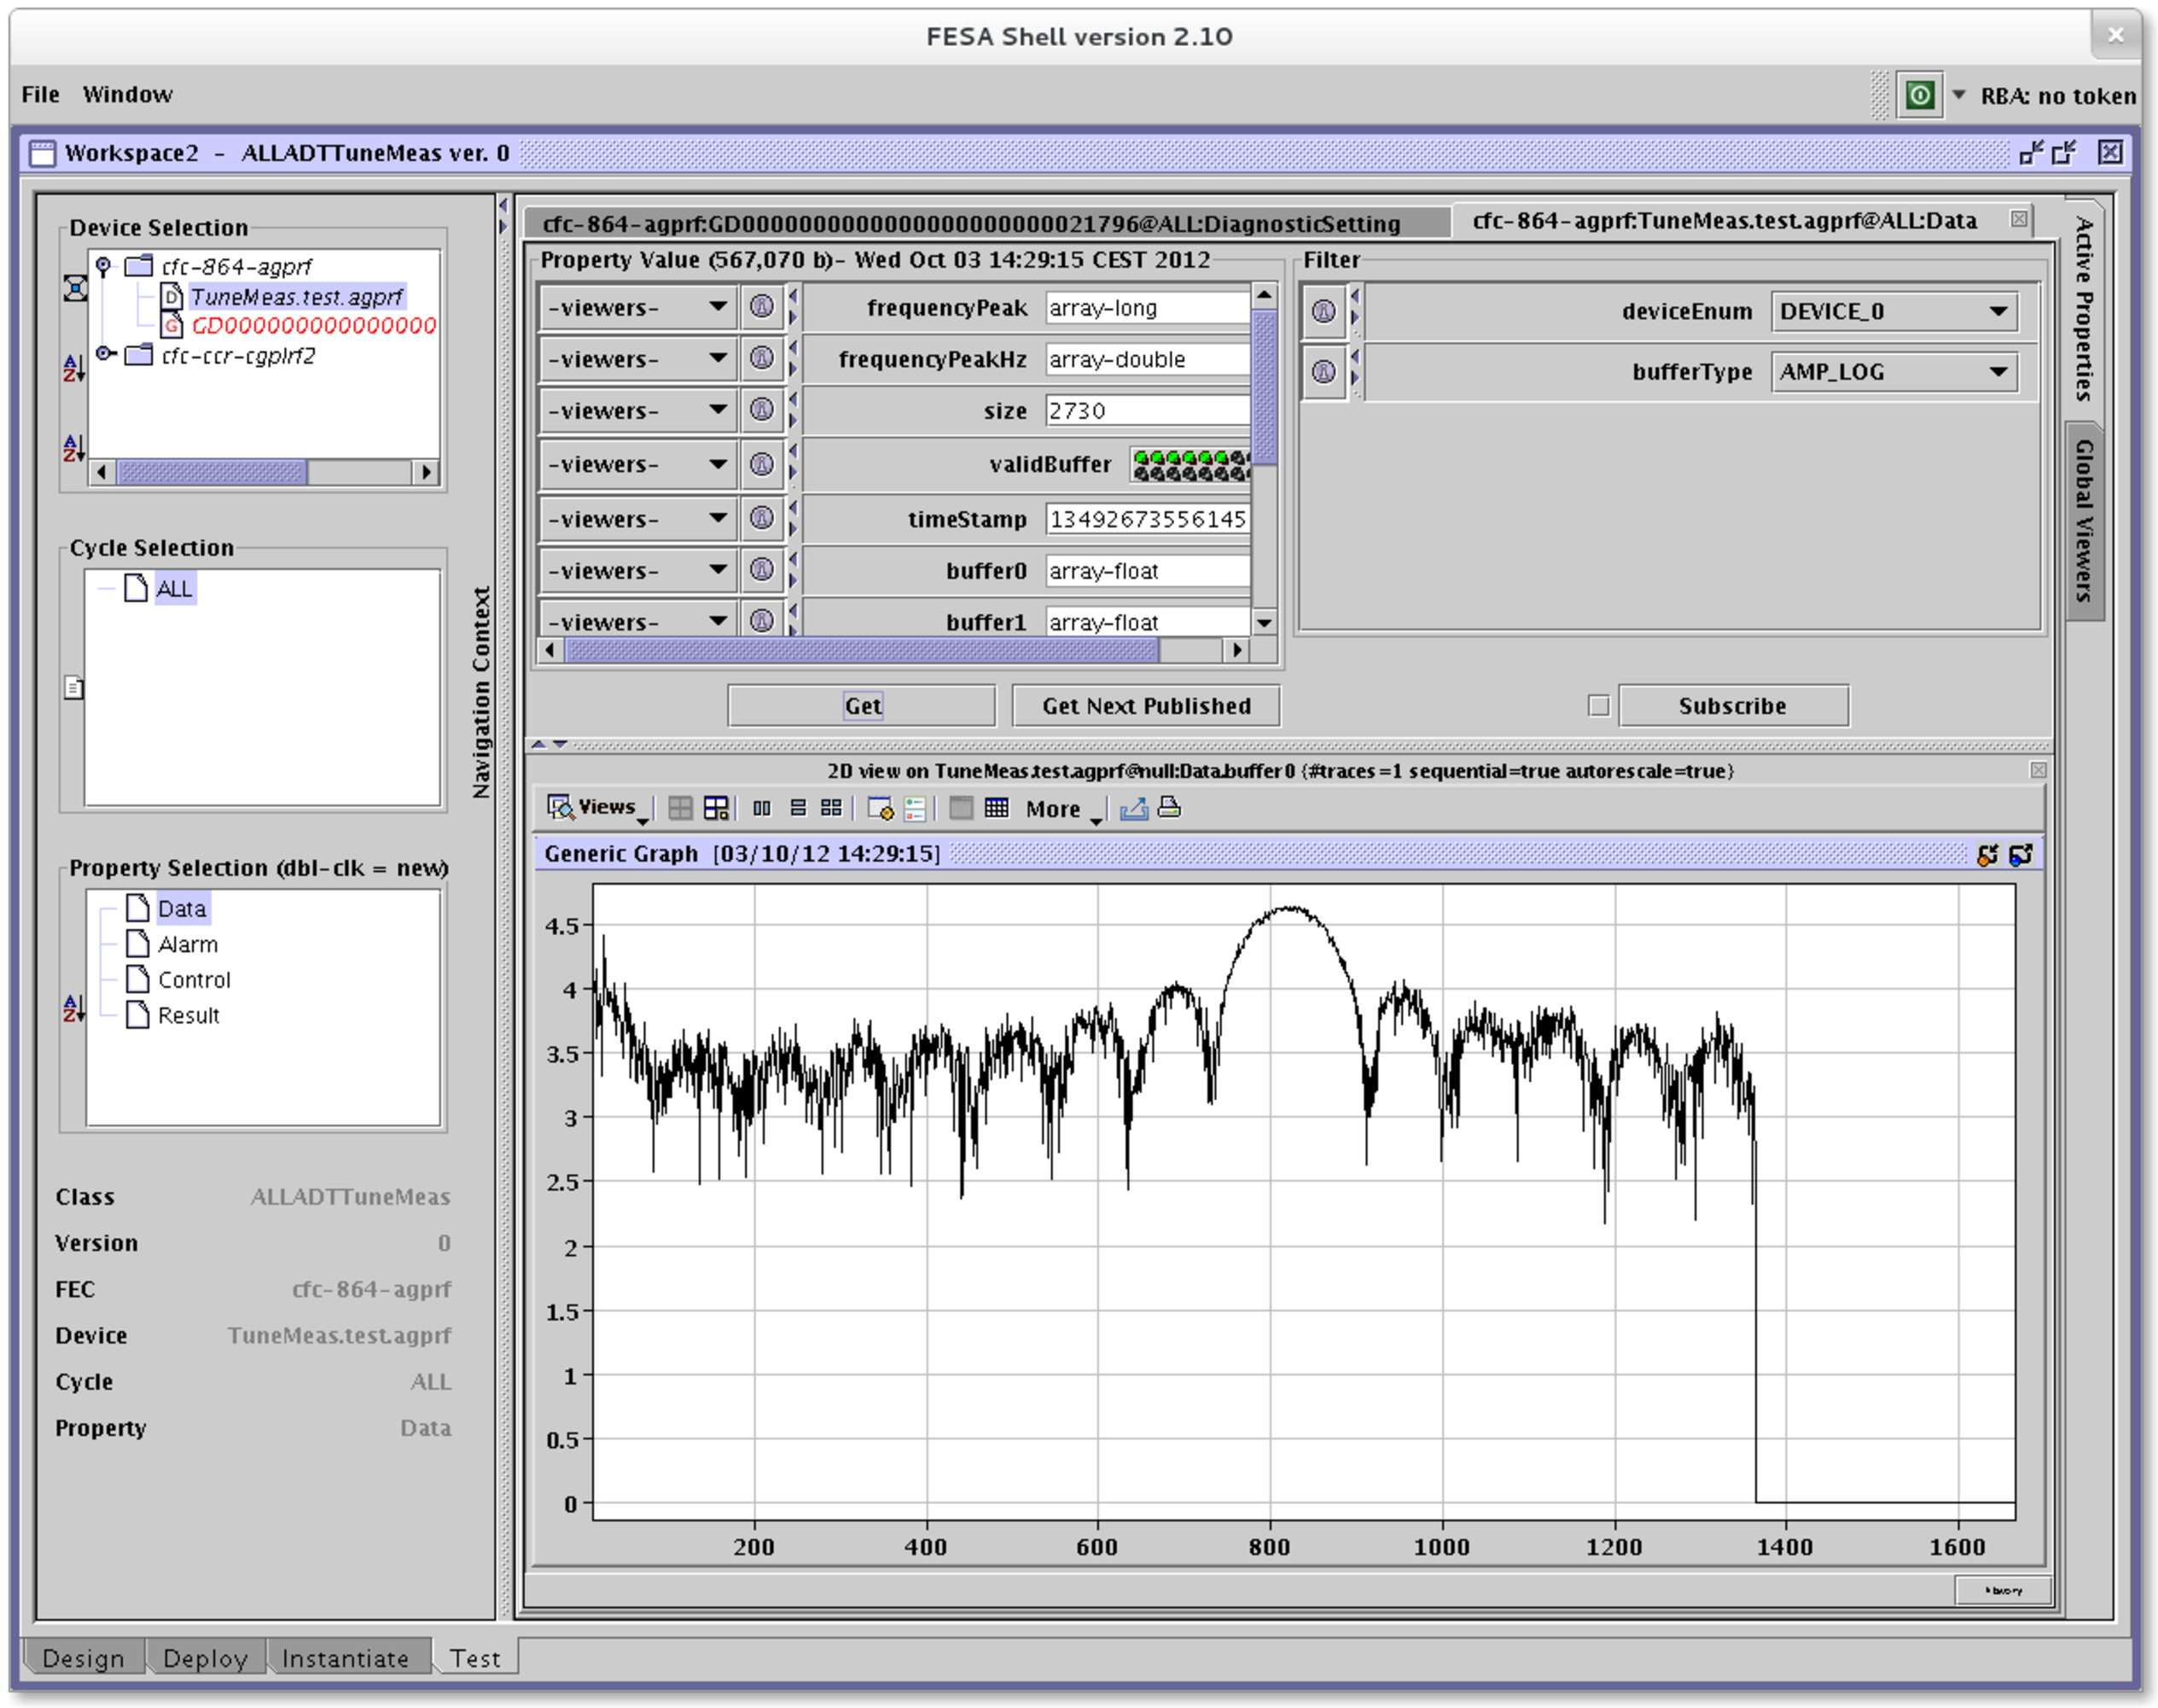
\includegraphics[scale=0.25]{amplitude_log.pdf}
\label{fig:tuneacq}
\end{figure}

From the control interface we can also via the data interface get access to the resulting graphs. We can choose which algorithm to use on the display~:

\begin{enumerate}
\item Time domain, that will display the raw signal.
\item Amplitude linear, that will display the amplitude of the FFT.
\item Amplitude logarithmic, same but on a log scale.
\item Average amplitude linear, averaging over all available bunches.
\item Average amplitude logarithmic, averaging over all available bunches logarithmic scale.
\item Phase, display the phase of the signal.
\end{enumerate}

The FFT and the Phase are computed using FFTW at the time of display. In fact this is using the same C++ \emph{bunch\_buffer} class than the one used in the data analysis software 

\subsection{ADTDSPU subscription}

\begin{figure}[H]
\caption{Tune measurement acquisition software in the FESA framework}
\centering
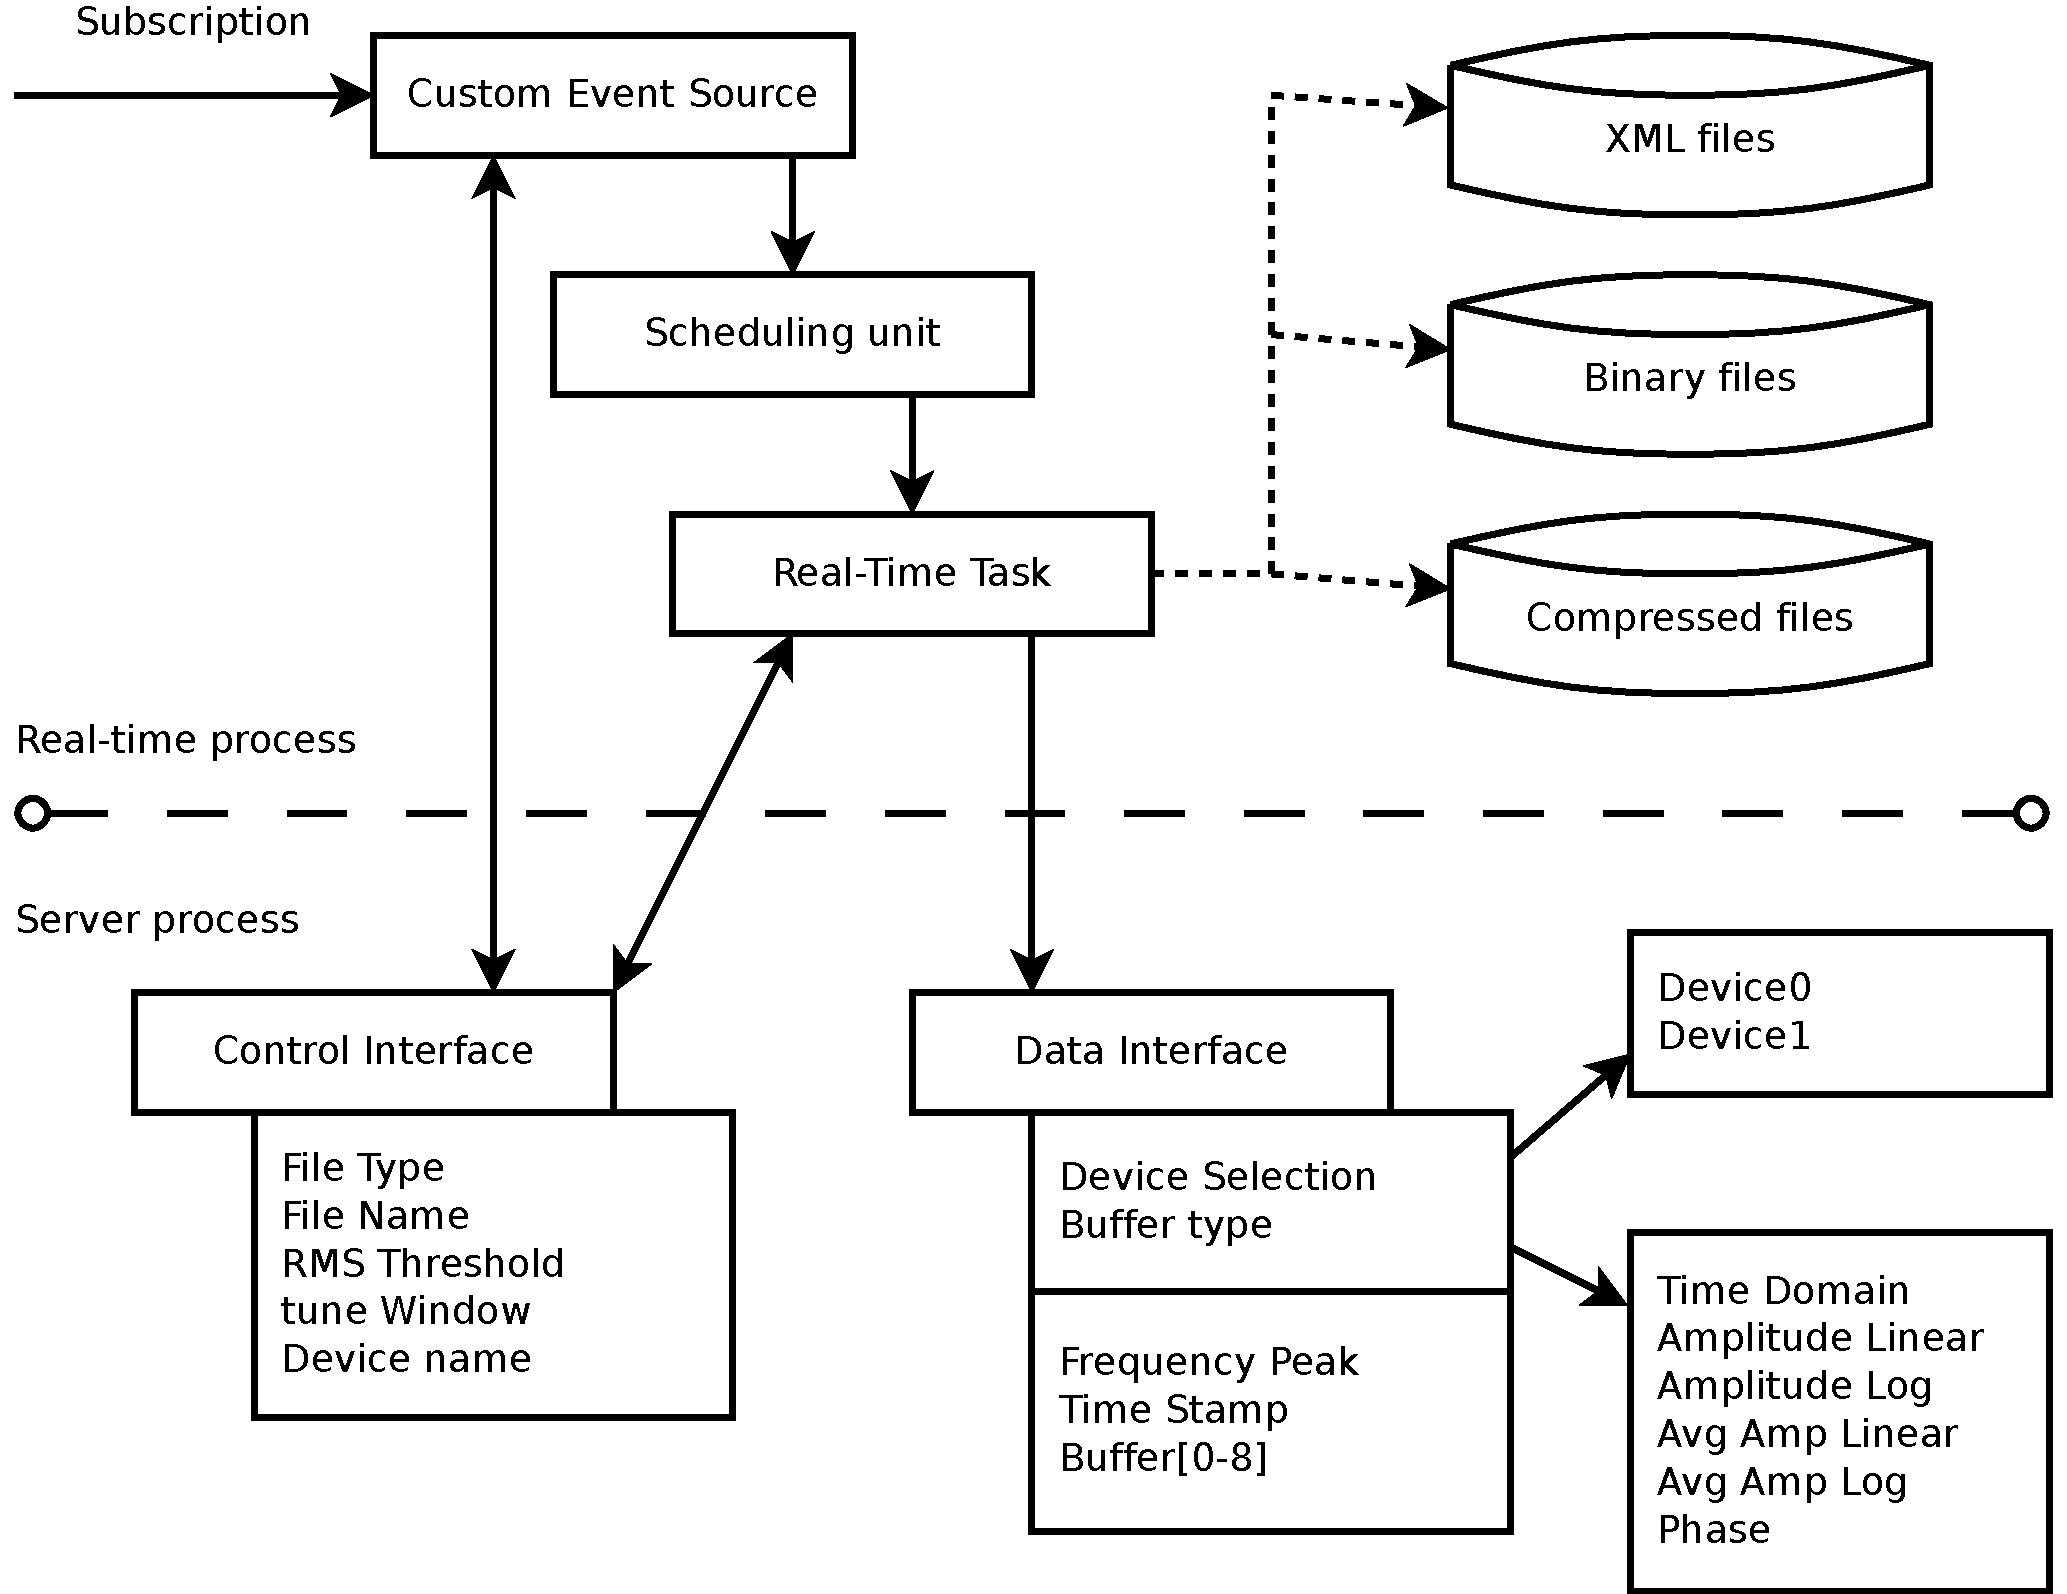
\includegraphics[scale=0.3]{tune_meas.pdf}
\end{figure}

The acquisition software uses the \gls{CMW}, a library used at \gls{CERN} to communicate between different layers of the accelerators control software, to connect to the \gls{ADTDSPU} control software and get the data when they are published (at the time of interrupt).

\section{Data analysis software}
\label{sec:data_analysis_software}

The data analysis software is a set of modules that can be enabled or bypassed to test the usefulness of an algorithm. The modularity of the data analysis software allow us to check the time taken by each part of the algorithm and validate it against the constraints.

\begin{figure}[H]
\caption{Time f\/low with different implementations and with 3000 bunches of 2048 points each.}
\centering
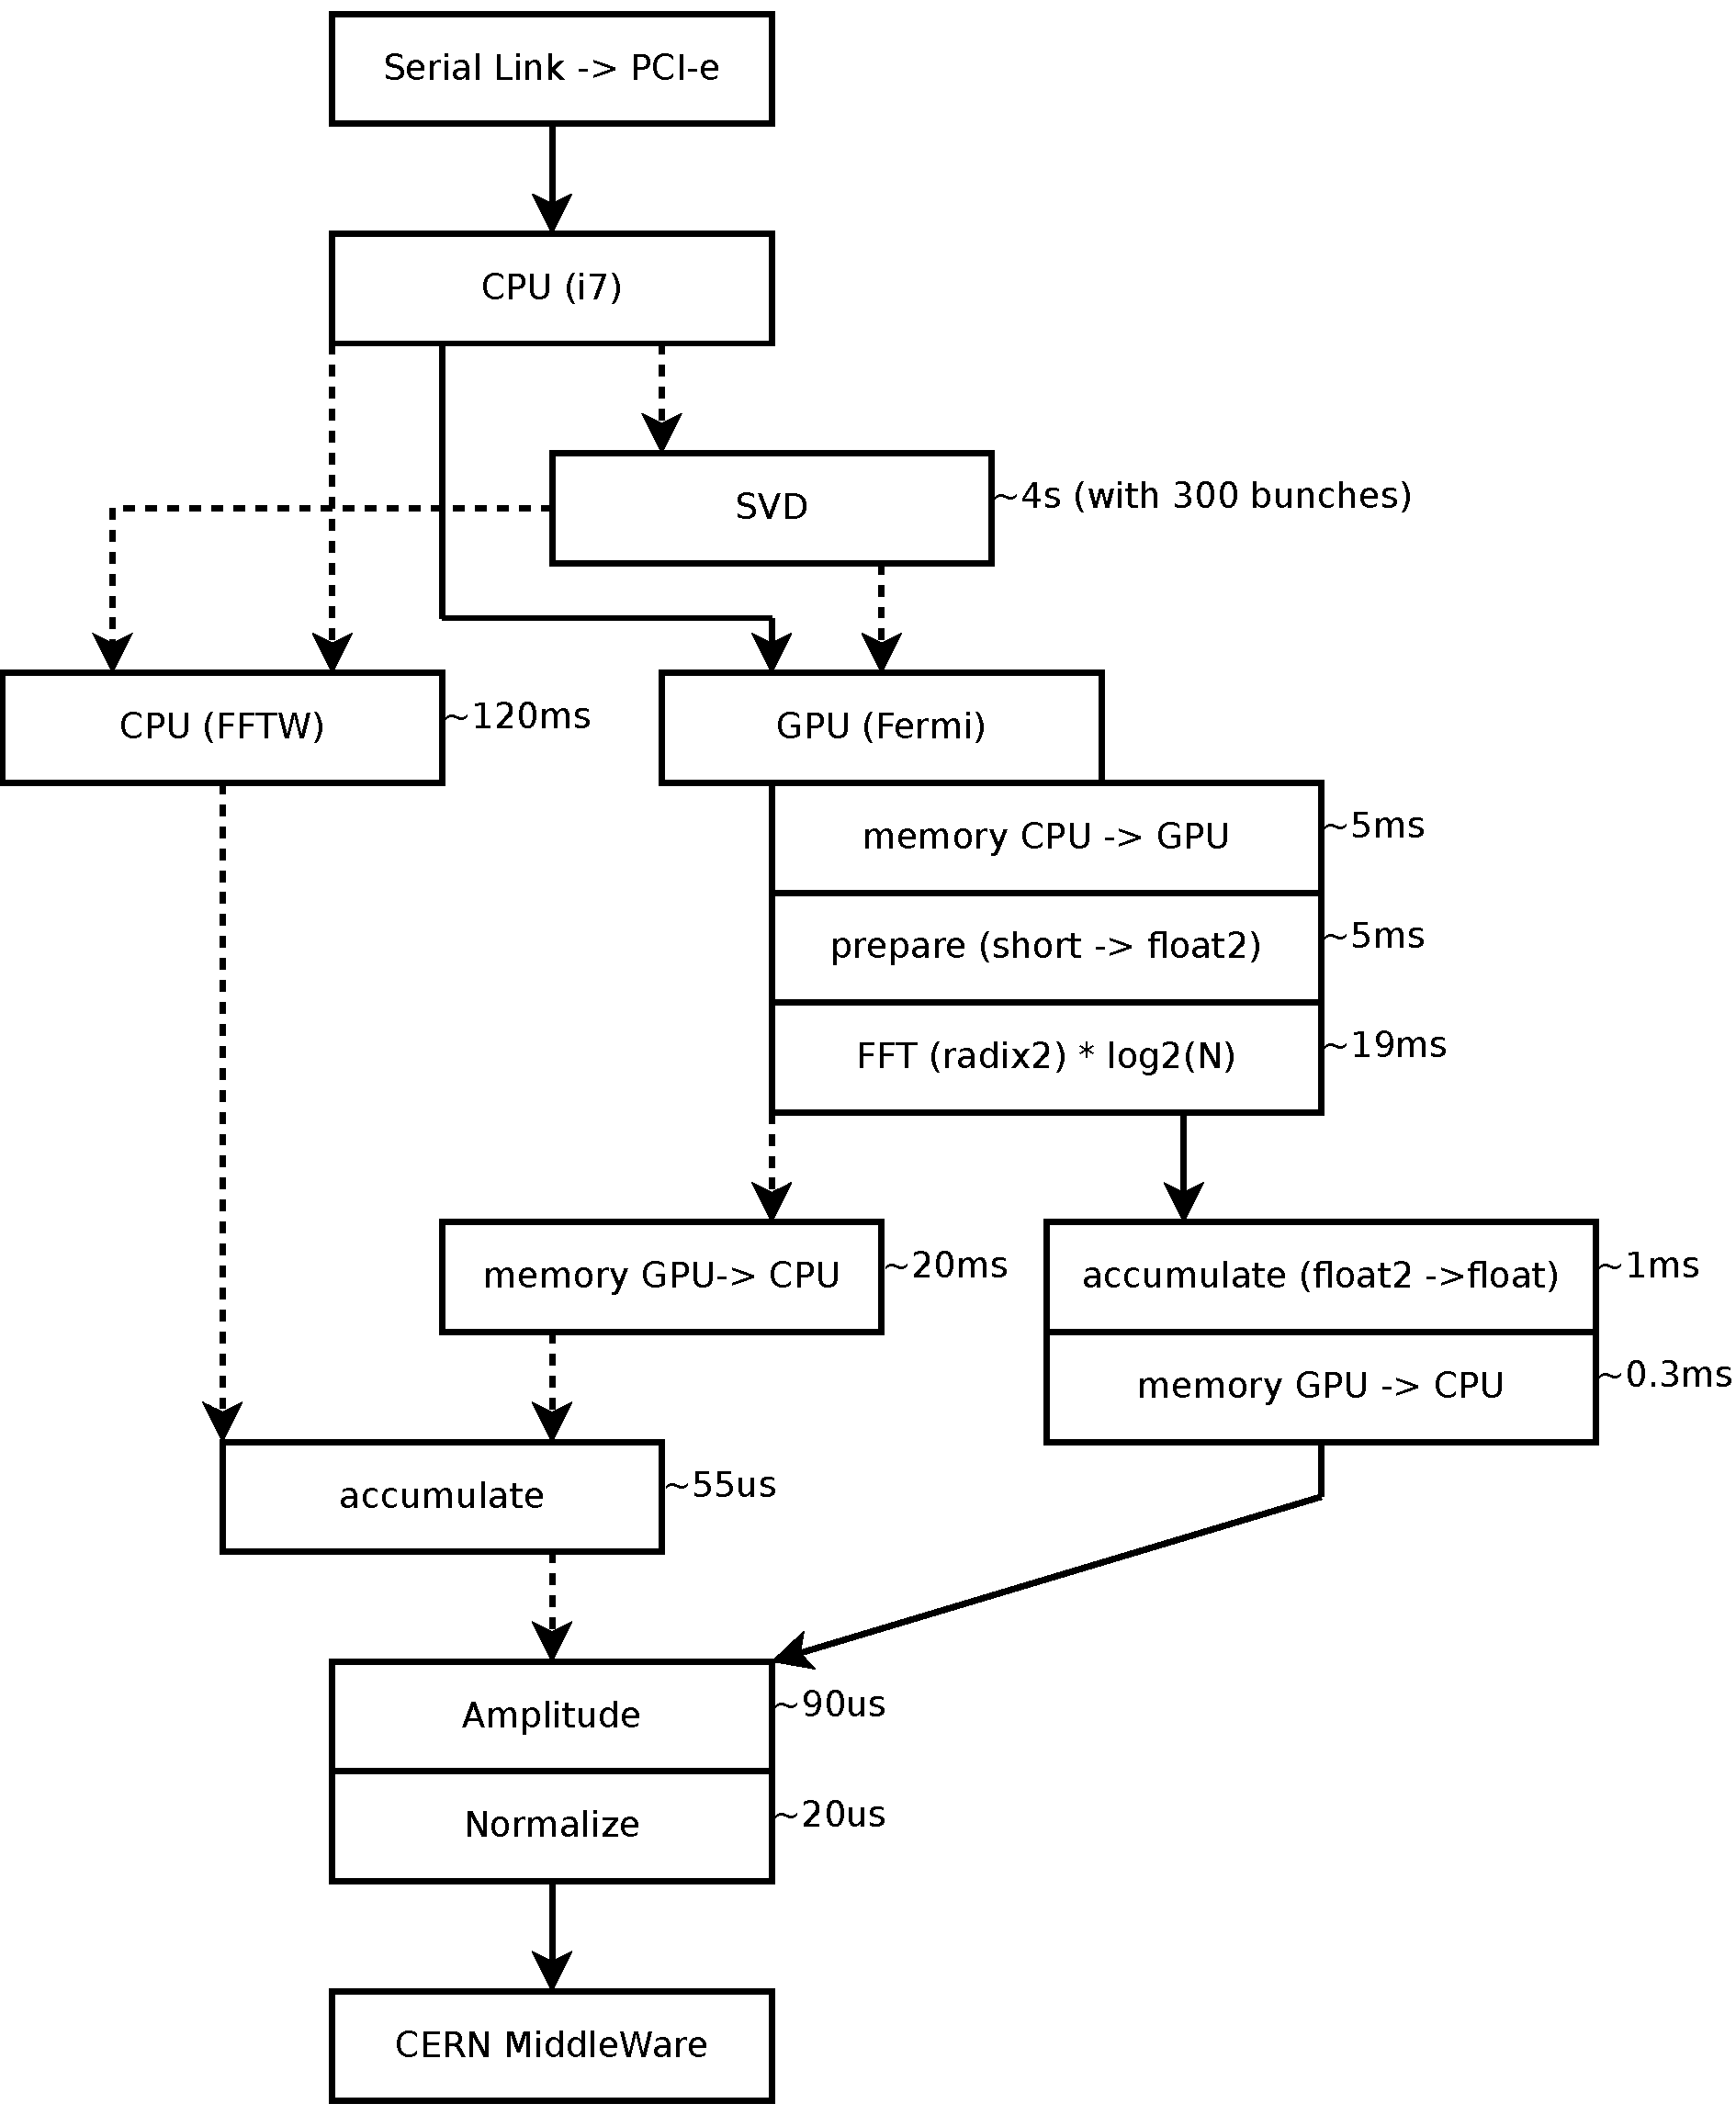
\includegraphics[scale=0.3]{PC-flow.pdf}
\label{fig:PCFlow}
\end{figure}

The \gls{FFT} are either computed on a \gls{GPU} or the \gls{CPU}, One could actually use \gls{OpenCL} on the \gls{CPU} and test the whole \gls{OpenCL} path. The different paths are due to memory copying, in the case of computations on the \gls{GPU}, one has to move the data from the \gls{CPU} central memory to the \gls{GPU} memory. This will be described in section~\ref{sec:FFT}.

To have a clear image and to combine the real and imaginary part of the \gls{FFT} we use the amplitude. It has been validated in the acquisition software as been the best metric, but could be changed at will in the final version. The amplitude is described in section~\ref{sec:amplitude}.

The accumulation over all theses bunches is done, which will give an average spectrum. The normalization step is only present for displaying the spectrogram (see section~\ref{sec:spectrogram}) and will not be needed for the final version.

\subsection{buffer management}

The data is first loaded from the files that were written by the
acquisition software. Buffers are loaded into the
\emph{acquisition\_buffer} class that are then collected together in
the \emph{bunch\_buffer} class. This class will use the interface to
\gls{FFT} (namely the abstract class \emph{i\_fft}) to compute the
\gls{FFT} using the method provided at instantiation.

\begin{figure}[H]
\centering
\caption{C++ buffer classes UML diagram}
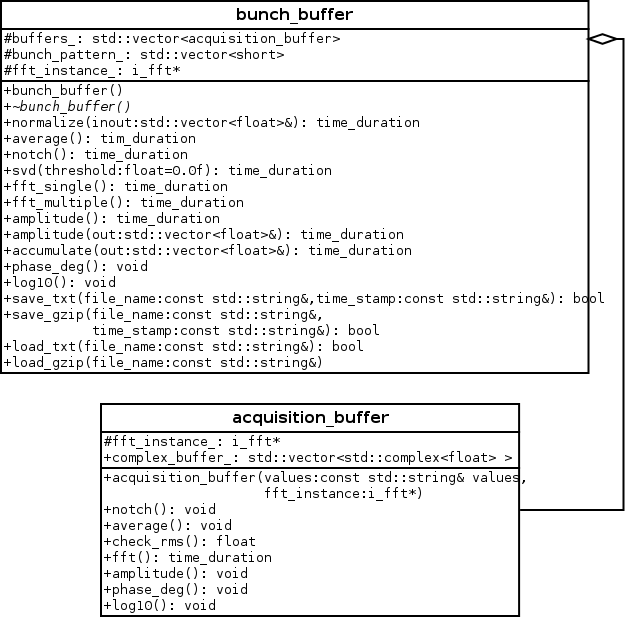
\includegraphics[scale=0.5]{buffer_uml.png}
\end{figure}

These classes are available in both single precision and double
precision versions. The version of the compiler available was not able
to support template correctly. The final version that will run on a
newer version of the Linux operating system should be able to handle
it, which will make the switch easier and at runtime.

It also contains all the various modules (apart from \gls{FFT}), some of which have their counterpart in \gls{GPU} code. This code is portable and used in both the tune measurement software and the data analysis software.

\subsection{FFT software architecture}

To be able to switch from \gls{FFTW} to the \gls{OpenCL} version of the \gls{FFT}, there is an abstract class that represents a \gls{FFT} transformation. It implements either \gls{FFTW} or \gls{OpenCL} version, as appropriate.

\begin{figure}[H]
\centering
\caption{C++ FFT classes UML diagram}
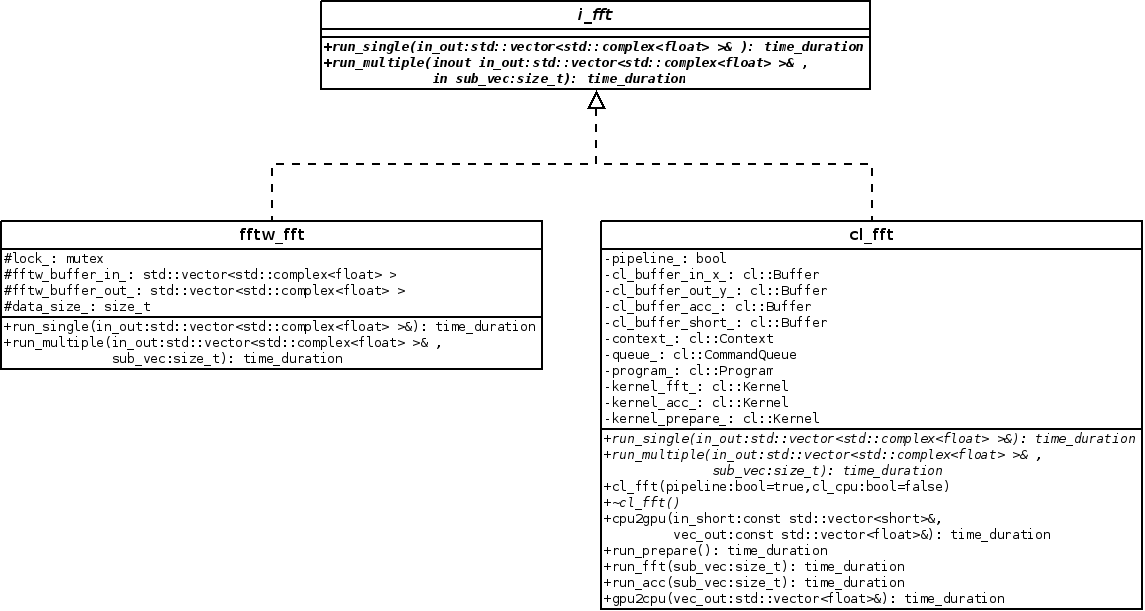
\includegraphics[scale=0.5]{fft_uml.png}
\end{figure}

The \gls{OpenCL} version is doing some steps of the algorithm in the \gls{GPU} itself. To avoid having to transfer to much data from the CPU to the GPU and to have to transform the data from the acquisition board (short 2 bytes integer) to the \gls{GPU} (single or double precision floating points) we do this step on the \gls{GPU} itself in the \emph{kernel\_prepare\_} kernel and then we do the \gls{FFT} computation in the \emph{kernel\_fft\_} kernel, finally we do the accumulation in the \emph{kernel\_acc\_}.

The \gls{OpenCL} \gls{FFT} use the algorithm described here~\cite{Govindaraju07}. The OpenCL Kernel is described here and composed of two part the twiddle and the main radix-2 part.

\begin{figure}[H]
\centering
\caption{OpenCL kernel code for the twiddle (used by FFT)}
\label{fig:twidle_cl}
\begin{lstlisting}
float2 twiddle(float2 a, int k, float alpha)
{
	float cs,sn;
	sn = sincos((float)k * alpha, &cs);
	return mul(a, (float2)(cs, sn));
}
\end{lstlisting}
\end{figure}

There is a difference between the \gls{FFT} described in the algorithm
cited above and the one seen here. Here the operation is parallized to
be made on multiples acquisitions at the same time, as in typical
operation we have to compute 2880 FFT at the same time. The thread is
multiplied by half the size of the acquisition and the number of
\glspl{FFT} to be made.

\begin{figure}[H]
\centering
\caption{OpenCL kernel code for multiple FFTs}
\label{fig:fft_cl}
\begin{lstlisting}
__kernel void fftRadix2Kernel(
	__global const float2 * x,
	__global float2 * y,
	const int p)
{
	// thread count
	int t = get_global_size(0);
	// thread index
  	int i = get_global_id(0);
	// fft index
  	int z = get_global_id(1);
  	// index in input sequence, in 0..P-1
  	int k = i & (p - 1);
  	// output index
  	int j = ((i - k) << 1) + k;
  	float alpha = -3.14159265359f * (float)k / (float)p;
  	
	// Read and twiddle input
	x += z * t * 2;
	x += i;
	float2 u0 = x[0];
	float2 u1 = twiddle(x[t], 1, alpha);
	
	// In-place DFT-2
	float2 tmp = u0 - u1; 
	u0 += u1; 
	u1 = tmp;
	
	// Write output
	y += z * t * 2;
	y += j;
	y[0] = u0;
	y[p] = u1;
}
\end{lstlisting}
\end{figure}

It is clear that the parallelization has a maximum equal in our case to half the number of samples $N$ / 2 multiplied by the number of \glspl{FFT}. On our test this mean 1024 * 2880, which is far more than the number of cores we can find on a top level \gls{GPU}, as is clear from table~\ref{tab:kepler}.

\subsection{SVD software}

An optional step is to apply a \gls{SVD} as described as suggested by Rama Calaga~\cite{PhysRevSTAB.7.042801} and by Wolfgang H{\"o}f\/le\cite{HofleChamonix12} which should reduce the noise in the signal (results are shown in section~\ref{sec:SVD}). The \gls{SVD} module is not visible here as it is a custom command (see figure~\ref{fig:spectrogram_uml}).

The \gls{GSL} was used to compute SVD from the available data. This means that technically the ``svd'' software should be under \gls{GPL}. A wrapper was also implemented to allow a more C++ style expression of the \gls{SVD} and make it more readable.

\begin{figure}[H]
\centering
\caption{SVD in the code (using C++ wrapper)}
\begin{lstlisting}
// M x N
gsl::matrix A(buffer_size(), bunch_count());
[...]
// N x N
gsl::matrix X(bunch_count(), bunch_count());
gsl::vector work(bunch_count());
gsl::vector S(bunch_count());
gsl::matrix V(bunch_count(), bunch_count());
gsl::matrix U = A;
// compute SVD
SVD_mod(U, X, V, S, work);
// S -> s
gsl::matrix s(bunch_count(), bunch_count());
for (size_t i = 0; i < bunch_count(); ++i) {
	if (S[i] < threshold) {
		s(i, i) = 0.0f;
	} else {
		s(i, i) = S[i];
	}
}
// vt = V^T
gsl::matrix vt = transpose(V);
// out = U s vt (out ~ A)
gsl::matrix out = U * s * vt;
[...]
\end{lstlisting}
\end{figure}

\Gls{GSL} offer different methods for calculating the \gls{SVD} of matrices, but the computing is only available in double precision float. The different approaches have different result varying with the size and shape of the matrix.

\subsection{Custom command and spectrograms}

On top of all these classes there is a general abstraction layer called \emph{commands} that decide what the software is going to execute on the buffers. Presently the commands are hard coded but we could in the future have a higher level languague decide which operation to do on the data. This could lead to a more flexible software to be used in operation.

\begin{figure}[H]
\centering
\label{fig:spectrogram_uml}
\caption{C++ spectrogram classes UML diagram}
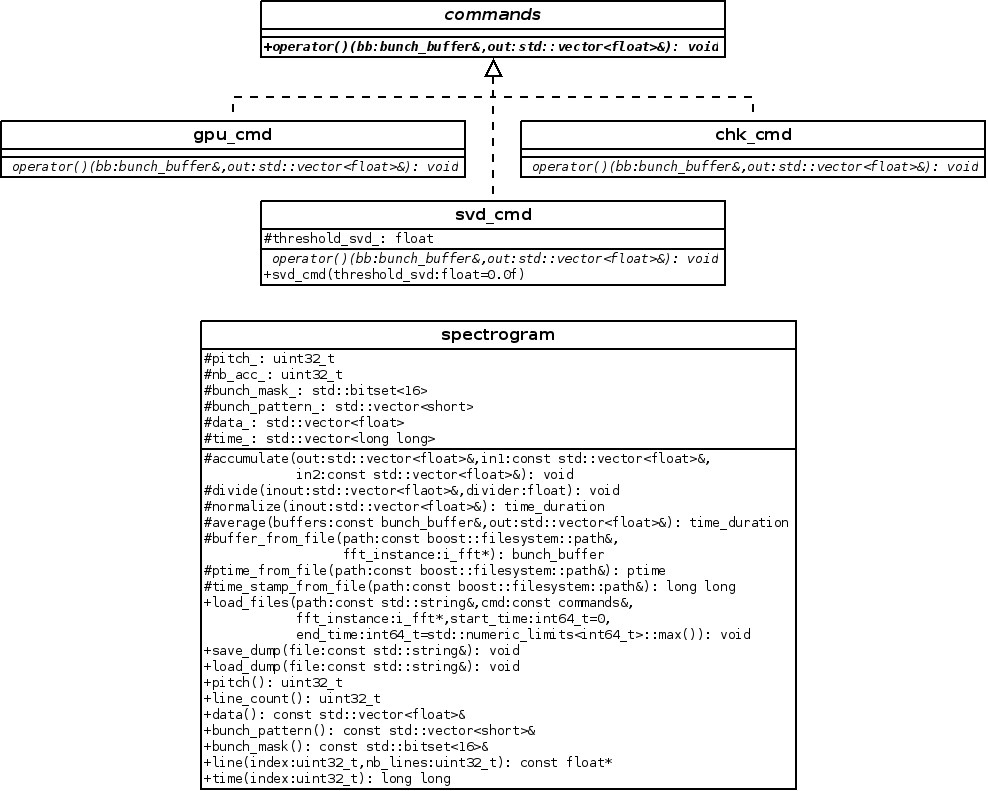
\includegraphics[scale=0.5]{spectrogram_uml.png}
\end{figure}

The spectrogram class is the class responsible for making the spectrogram from the buffers and to add timestamps and values. It uses \gls{OpenCV} as an image library. There is also a possibility to display the spectrogram directly using \gls{OpenGL}/GLUT.


